\documentclass[11pt]{article}    
\usepackage[a4paper,left=1in,right=1in,top=1in,bottom=1in]{geometry} 

\usepackage[english]{babel}
\usepackage[T1]{fontenc} 
\usepackage[utf8]{inputenc}
\usepackage{seqsplit}

\renewcommand{\familydefault}{\sfdefault} 
\usepackage{setspace}  \singlespacing  
\usepackage{graphicx}        
\usepackage[absolute]{textpos}
\usepackage{xcolor}
\usepackage{fontawesome5}
\usepackage{multirow}
\usepackage{hyperref}
\usepackage{tcolorbox}
\hypersetup{
    colorlinks,
    linkcolor={red!50!black},
    citecolor={blue!50!black},
    urlcolor={blue}
}

\definecolor{mgray}{gray}{0.85}
\definecolor{mpurple}{HTML}{68236D}
% Additional packages for the content
\usepackage{float}
\usepackage{subfig,wrapfig}
\usepackage{amsmath,amsfonts,amsthm,amssymb}
\usepackage{fancyhdr,fancybox,color}
\usepackage{enumerate}
\usepackage[amssymb]{SIunits}
\definecolor{MyBlue}{rgb}{0,0.3,0.6}
\usepackage[all]{hypcap}
\usepackage{csquotes}
\usepackage[url=false,
backend=bibtex,
style=authoryear-comp,
doi=true,
isbn=true,
backref=false,
dashed=false,
maxcitenames=2,
maxbibnames=99,
natbib=true]{biblatex}
\DeclareNameAlias{author}{family-given}
\renewbibmacro{in:}{}
\addbibresource{../_logosAndRef/references.bib}
\nonfrenchspacing

% Configurable separation between header and body
\newlength{\headertobodysep}
\setlength{\headertobodysep}{1cm}

% Header with logos and contact information
\begin{document}
\thispagestyle{empty}

% Lean header with aligned elements
\textblockorigin{0pt}{0pt}

% Durham logo on the left
\begin{textblock*}{5cm}(0.5cm,1cm)
    
\includegraphics[height=2cm]{../_logosAndRef/Durham-University.pdf}
\end{textblock*}

% Contact information in the center - vertically centered with logos
\begin{textblock*}{9cm}(6cm,1.5cm)
    \centering
    {\large \textbf{Sneezing droplets | CoMPhy Lab}}\\[0.2em]
    Department of Physics, Durham University\\[0.3em]
    \href{https://comphy-lab.org}{comphy-lab.org}
\end{textblock*}

% CoMPhy logo aligned with right margin
\begin{textblock*}{5cm}(15.5cm,1cm) % exactly 1 cm away from the right edge
    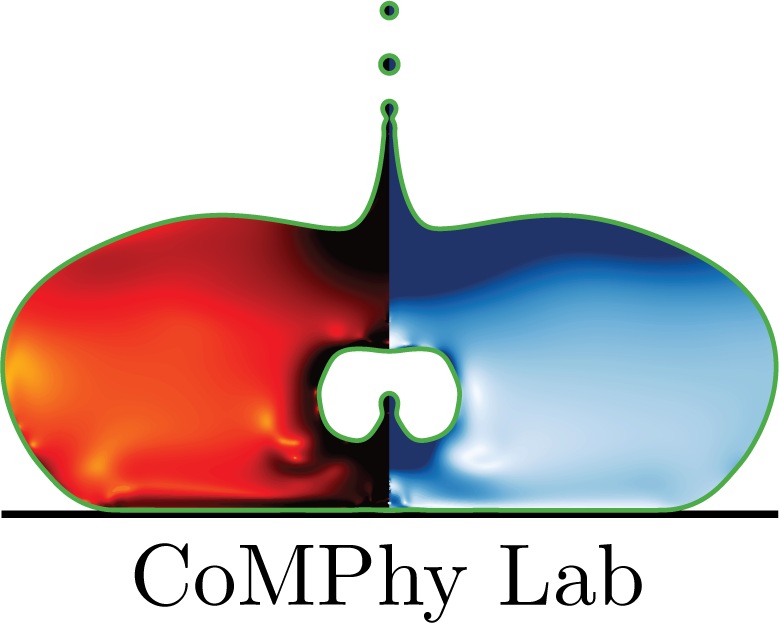
\includegraphics[height=2cm]{../_logosAndRef/CoMPhy-Lab.png}
\end{textblock*}

% Reset to normal text flow after header
\vspace*{\headertobodysep}

\begin{center}
    \begin{LARGE}
        Sneezing droplets: Modeling of respiratory droplet formation
    \end{LARGE}
\end{center}

\noindent Ever wondered why a sneeze produces such a specific pattern of droplets? The physics behind this everyday phenomenon holds keys to understanding airborne disease transmission.

\begin{tcolorbox}[colback=mgray,colframe=mpurple,title=TL;DR]
    Understanding droplet distributions from respiratory actions remains a key scientific challenge. While Newtonian fluid breakup under airflow is well understood, human respiratory fluids exhibit viscoelastic behavior that fundamentally alters these dynamics. This project numerically investigates how viscoelasticity affects filament breakup -- the second stage of droplet formation where liquid filaments fragment into individual droplets. Using state-of-the-art computational fluid dynamics, we will simulate viscoelastic filament dynamics and compare results with existing Newtonian data to isolate elasticity's role. The findings will improve droplet size distribution predictions during respiratory events, informing airborne disease transmission mitigation strategies.
\end{tcolorbox}

\section*{Description}

During the COVID-19 pandemic, many of us wondered how viruses are transmitted from one person to another. It turns out that when we cough, sneeze, or speak, we produce numerous droplets that play a crucial role in spreading these viruses \citep{bourouiba2021fluid}. Understanding droplet distributions from respiratory actions remains a key scientific challenge. While Newtonian fluid breakup under airflow is well understood, human respiratory fluids exhibit viscoelastic behavior that fundamentally alters these dynamics. This project numerically investigates how viscoelasticity affects filament breakup -- the second stage of droplet formation where liquid filaments fragment into individual droplets. Using state-of-the-art computational fluid dynamics, you will simulate viscoelastic filament dynamics and compare results with existing Newtonian data to isolate elasticity's role. The findings will improve droplet size distribution predictions during respiratory events, informing airborne disease transmission mitigation strategies.

\begin{figure}
    \begin{center}
     \includegraphics[width=\textwidth]{sneeze.png}
     \caption{Stages of sneeze ejecta as experimentally reported by \citet{scharfman2016visualization}. One can notice several long filaments breaking up into droplets.}
     \label{Figure::Typical}
    \end{center}
    \end{figure}
    
    \begin{figure}
        \begin{center}
            \includegraphics[width=\textwidth]{filament_01.pdf}
            \caption{(a) Sketch of the initial filament, and (b) the final shapes obtained for different values of filament length $L_0$, studied for Newtonian fluids by \citet{anthony2019dynamics}. }
            \label{fig:filament}
        \end{center}
    \end{figure}
\section*{Deep dive}

From a physics perspective, coughing or sneezing can be understood as airflow over a thin liquid layer attached to a surface \citep{kant2023bag}. This phenomenon is well understood for Newtonian fluids. However, this understanding does not apply well to human coughs, as mucosalivary fluids exhibit non-Newtonian (viscoelastic) behavior. Consequently, we lack a comprehensive understanding of the influence of non-Newtonian effects on the overall dynamics. We have recently made efforts to understand the non-Newtonian effects of jet breakup (see \citet{dixit2024viscoelastic,liViscoelasticityReducesDroplet2025}).

During coughing, breakup of mucosalivary fluids into droplets occurs in two steps. The first step involves breaking liquid sheets into filaments, while the second step involves breaking those filaments into droplets. For Newtonian liquids, the overall dynamics are governed by competition among three physical effects: capillarity, viscosity, and inertia \citep{anthony2019dynamics}. However, for mucosalivary fluids, which display viscoelastic properties, elasticity also plays a crucial role \citep{sen2021retraction, liu2022contraction}. Understanding these dynamics, along with the resulting droplet size, is essential for analyzing sneeze droplets and developing effective strategies to mitigate airborne disease transmission.

You will numerically study the dynamics of viscoelastic filament breakup into droplets (see figure \ref{fig:filament}). We will examine the overall dynamics and droplet size and compare our results with existing data on Newtonian fluids \citep{anthony2019dynamics}. Finally, we will apply our analysis to understand droplet distribution during coughing or sneezing. 

\section*{What you will do and what you will learn?}
% The project will focus on the following:
\begin{enumerate}
\item You will learn about the physics of fluids, and science underlying non-Newtonian fluid flows. 
\item You will learn how to utilize computational tools to study real life physics. 
\item You will learn how to collaborate with a diverse group of researchers, specifically with other experimentalists and theoreticians.
\item You will have access to a read-to-use codebase (available on \href{https://github.com/comphy-lab/multirheoflow}{GitHub}).
\item As a part of the \href{https://comphy-lab.org}{CoMPhy lab}, you will learn and adapt open-source coding principles. 

\end{enumerate}

If you have any questions, feel free to contact us \href{mailto:vatsal.sanjay@comphy-lab.org}{vatsal.sanjay@comphy-lab.org}/\\\href{mailto:vatsal.sanjay@durham.ac.uk}{vatsal.sanjay@durham.ac.uk} or drop by Ph255 (Rochester building) at the Department of Physics at Durham University.

\begin{center}
\begin{tabular}{|l|l|l|}
\hline \textbf{Collaborators} & \textbf{E-mail} & \textbf{Based at} \\
\hline \multirow{2}{*}{Dr. Vatsal Sanjay} & \href{mailto:vatsal.sanjay@comphy-lab.org}{vatsal.sanjay@comphy-lab.org} & \multirow{2}{*}{Ph255 (Rochester building)} \\
& \href{mailto:vatsal.sanjay@durham.ac.uk}{vatsal.sanjay@durham.ac.uk} & \\
\hline Ayush Dixit M.Sc. & \href{mailto:a.k.dixit@utwente.nl}{a.k.dixit@utwente.nl} & Univ. Twente \\
\hline Adj. Prof. Alvaro Marin & \href{mailto:a.marin@utwente.nl}{a.marin@utwente.nl} & Univ. Twente \\
\hline Prof. Dr. Detlef Lohse F.R.S. & \href{mailto:d.lohse@utwente.nl}{d.lohse@utwente.nl} & Univ. Twente  \\
\hline
\end{tabular}
\end{center}

\vspace{1em}
\noindent\textit{Last updated: \today}

\printbibliography
\end{document}